\chapter{Испытание и обоснование эффективности предлагаемых подходов}
\section{Проектирование ПО}
Разработанное программное обеспечение дожно соответствовать техническому заданию представленное в Приложении Б и должна обеспечивать возможность выполнения следующих ниже функций:
\begin{enumerate}
    \item Предоставлять возможность сохранять и загружать данные используемые для работы программы:
    \begin{itemize}
        \item загрузка данных пользователей о перемещении;
        \item преобразование загруженных данных во внутренний формат программы;
        \item сохранение расчётных данных для последующей обработки;
    \end{itemize}
    \item Предоставлять функцию кластеризцаии по заданным параметрам, включающая следующие пункты:
    \begin{itemize}
        \item использование заданной метрики;
        \item ограничение на количество итераций алгоритма;
        \item способ расстановки начальных кластеров.
    \end{itemize}
    \item Предоставлять возможность визуализировать выходные данные.
\end{enumerate}

Предложенные алгоритмы из разделов \ref{sec:kmeans} и \ref{sec:distance} были реализованы с использованием языка программирования Python и сервиса построения маршрутов Open Source Routing Machine для расчета расстояния между узлами графа по городским дорогам. Программный код опубликован на хостинге Github (подробнее в Приложении~А).

\section{Методика проведения эксперимента}
Для оценки эффективности работы алгоритма и изучения специфики метрики Route были проведены эксперименты, в ходе которых менялись выборки данных, количество получаемых кластеров и их начальное местоположение, а так же реализация метода.

Для генерации данных о предпочтениях жителей города по перемещению был создан инструмент Scatter~\cite{scatter}, позволяющий удобным образом генерировать большие объемы геоданных.

Для оценки работы алгоритма на данных, приближенных к реальным, были сгенерированы данные о предпочтениях по перемещению жителей среднего по размерам города с примерным числом жителей около 350 000. В качестве результата было получено 6000 пар точек отправления--назначения (рис.~\ref{pic:full}), или 12000 точек в общей сложности (выборка Main). Эту выборку было решено разбить на 125 кластеров, начальное положение которых было случайным. В последствие это случайное расположение кластеров было взято за основу для тестирования различных версий алгоритма.

\begin{figure}[ht!]
    \centering
    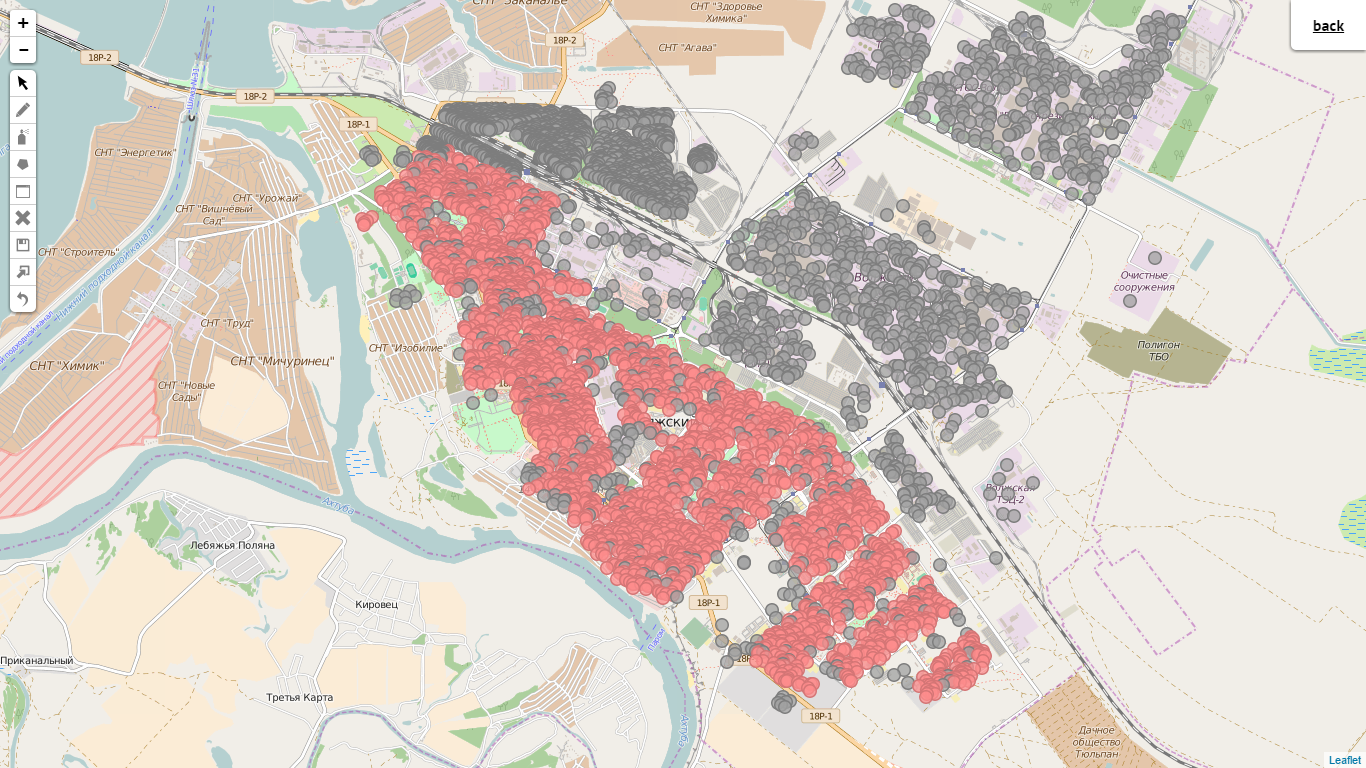
\includegraphics[width=.9\textwidth]{full} \\[1ex]
    \parbox{.9\textwidth}{\caption{Сгенерированная выборка из 12000 точек. Красным отмечены точки отправления, серым~--- назначения} \label{pic:full}}
    \vspace*{-1ex}
\end{figure}

\begin{figure}[b!]
    \centering
    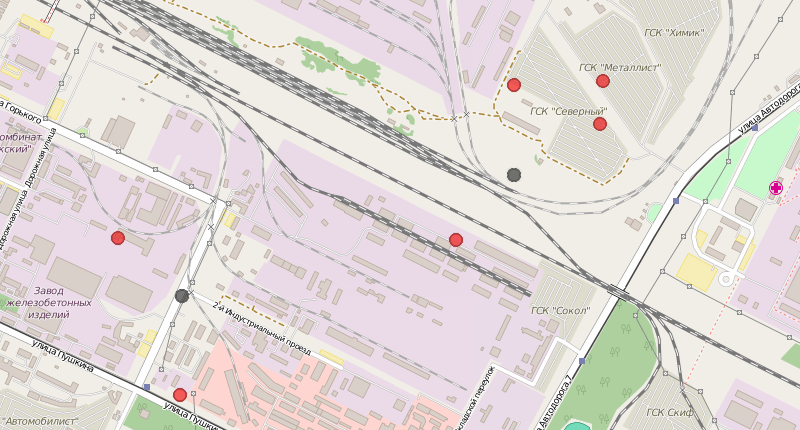
\includegraphics[width=.47\textwidth]{test_railway-contrast}\
    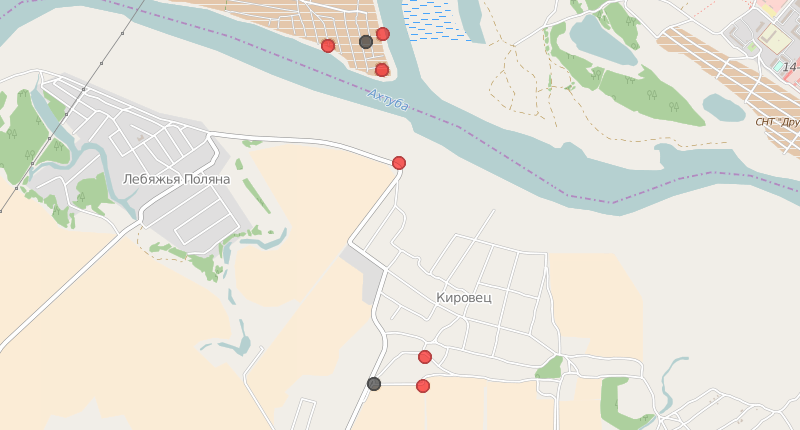
\includegraphics[width=.47\textwidth]{test_river-contrast} \\
    \parbox{.47\textwidth}{\small\centering a)}\ \parbox{.47\textwidth}{\small\centering б)}
    \parbox{.9\textwidth}{\caption{Выборки для проверки обхода препятствий. На рисунке а) между объектами выборки находится железная дорога, на рисунке б)~--- рек. Красными кругами отмечены элементы выборки, черными~--- начальные центры кластеров} \label{pic:railway-river}}
    \vspace*{-1ex}
\end{figure}

Так же были сгенерированы другие выборки для проверки специфичных случаев: обхода препятствий в виде железной дороги (выборка Railway, рис.~\ref{pic:railway-river}а) и реки (выборка River, рис.~\ref{pic:railway-river}б). Каждая из них представляет собой набор из шести точек, которые кластеризуются в два кластера. Точки и начальные центры расположены таким образом, что если алгоритм не учитывает препятствия между объектами выборки, то в одном кластере окажутся точки, разделенные препятствием.

Критериями для оценки эффективности разработанных алгоритмов и метрик являются:
\begin{itemize}
    \item время, затраченное на расчет расстояния между объектами выборки;
    \item учет препятствий;
    \item визуальная оценка результатов кластеризации.
\end{itemize}
